\scanpage{40}
% archive sheet number: 39
\noindent\makebox[0pt][r]{\rule[-1.4ex]{.4pt}{3.7ex}\hspace{.5em}}\uline{Proposition} Soi\deleted{\unsure{ent|t}}t $(C,\sigma,<)$ une \unsure{maquette|moquette} ordonnée. Alors pour tt $x\in C$, les \deleted{\unsure{ens.|sous}} ens.
\[
\begin{aligned}
 C_{\geq x}&=\{y\in C\mid y\geq x\}\\
 C_{\leq x}&=\{y\in C\mid y\leq x\}
\end{aligned}
\]
\makebox[0pt][r]{\rule[-.4ex]{.4pt}{2.4ex}\hspace{.5em}}sont \uline{tot\textsuperscript{\unsure{t|l}}} ordonnés.

Il suffit de \inserted{le} prouver \inserted{pour} \unsure{\deleted{le}|le|\deleted{la}} premier \raisebox{1.3ex}{\unsure{.}\deleted{\unsure{notons|noter}}} (par dualité), \deleted{Soit \unsure{donc}} \unsure{cel|cela} signifie \unsure{aussi|ceci} :
\[
\begin{aligned}
 &\text{Si}\quad x<y,\quad x<z,\quad \text{avec}\quad y\ne z\\
 &\hspace{1em}\text{alors}\quad (y,z)\ \text{comparables.}
\end{aligned}
\]

\noindent\begin{minipage}[c]{.34\linewidth}
\figure{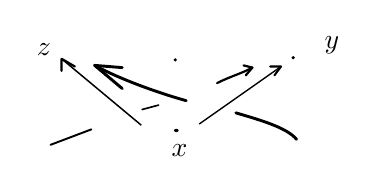
\begin{tikzpicture}[x=.014cm,y=-.014cm,line cap=round,line join=round]
\node at (31,35) {$z$};
\node at (292,31) {$y$};
\node at (154,126) {$x$};
\fill (150,44) circle[radius=.65pt];
\fill (257,42) circle[radius=.65pt];
\fill (151,108) ellipse[x radius=.85pt,y radius=.6pt];
\draw[line width=.55pt] (119,103) -- (47,43);
\draw[line width=.8pt] (47,54) -- (47,43) -- (59,50);
\draw[line width=.5pt] (172,102) -- (246,50);
\draw[line width=.75pt] (236,50) -- (246,50) -- (240,58);
\draw[line width=1.05pt] (160,81) .. controls (135,74) and (101,62) .. (77,49);
\draw[line width=1.05pt] (102,51) -- (77,49) -- (102,70);
\draw[line width=.8pt] (188,65) .. controls (200,59) and (211,56) .. (220,51);
\draw[line width=.8pt] (212,49) -- (220,51) -- (214,58);
\draw[line width=.7pt] (37,121) -- (74,107);
\draw[line width=.6pt] (120,89) -- (135,85);
\draw[line width=1.05pt] (205,92) .. controls (225,98) and (251,105) .. (260,116);
\end{tikzpicture}}
\end{minipage}\hfill\begin{minipage}[c]{.63\linewidth}
[On note que $y$ et $z$ sont non congrus mod $\sigma$, à cause de 28 a),]
\end{minipage}

Si $\unsure{\deleted{x}}y$ et $\unsure{\deleted{y}}z$ étaient incomparables; on aurait que $\sigma y$ et $z$ sont comparables, On \unsure{peu|pas|ne} peut avoir $z\leq\sigma y$ car on. aurait $x\leq\sigma y$, ce qui contredit $x<y$ par (28) a). On \deleted{\unsure{ne peut avoir}} \inserted{aurait donc} $\sigma y<z$ d'où $\sigma z<\unsure{\backslash|x}$

\clearpage
